\documentclass[a4paper,12pt,one side,titlepage]{report}


%en francais
\usepackage[T1]{fontenc}
\usepackage{lmodern}
\usepackage[utf8]{inputenc}
\usepackage[francais]{babel}



\usepackage{listings}
\usepackage{geometry}
\usepackage{graphicx}
\usepackage{eurosym}
\usepackage{url}
\usepackage{pdfpages}
\usepackage[acronym]{glossaries}
\usepackage{hyperref}
\usepackage{graphicx}
%\usepackage[top=2.5cm,bottom=2.5cm,left=2.5cm,right=2.5cm]{geometry}
%\hypersetup{pdfborder=0}




\newglossaryentry{firewall}
{
	name={firewall},
	description={Protection pour serveur}
}

\newglossaryentry{naxsi}
{
	name={naxsi},
	description={Un type de firewall}
}



\makeglossaries
\begin{document}
%\includepdf[pages = {1-1}]{./pdf/1stpage.pdf}
%\includepdf[pages = {1-1}]{./pdf/pagegarde.pdf}


\begin{titlepage}
\begin{center}

\textsc{\LARGE Licence ASRALL}\\[1.5cm]

\textsc{\Large Exposé technique}\\[5.9cm]

% Title
{ \huge \bfseries Fully Automatic Installation\\[1.9cm] }

% Author and supervisor
\noindent
\begin{minipage}{0.4\textwidth}
\begin{flushleft} \large
François \textsc{Dupont}
\end{flushleft}
\end{minipage}%
\begin{minipage}{0.4\textwidth}
\begin{flushright} \large
Florent \textsc{Fillion}
\end{flushright}
\end{minipage}

\vfill

% Bottom of the page
{\large \today}

\end{center}
\end{titlepage}


%Page table des matières
\tableofcontents

%Introduction
\chapter{Introduction}
\section{Objectifs}
\subsection{Définition}
\textit{Fully Automatic Installation} ou \textsc{FAI} est un logiciel libre, inspiré de son équivalent \textsc{Solaris}, \textsc{Jumpstart}. Il permet d'installer et de configurer un système d'exploitation Linux sur une ou plusieurs machines, en utilisant un infrastructure client serveur, de façon rapide et automatisé.

Il est à noter que \textsc{FAI} n'est pas interactif contrairement à d'autres logiciels remplissant sensiblement la même fonction. Ce logiciel est également considéré comme mature puisqu'il en est à sa 4\textsuperscript{ème} itération majeure (4.0) et est développé de façon continue depuis 1999.

\subsection{Utilité}
\textsc{FAI} s'adresse particulièrement aux administrateurs ayant à gérer un grand parc de machine sous Linux, que ce parc soit \textit{virtualisé} ou physique (et même des \textit{chroot}s).
On peut citer EDF qui a récemment utilisé FAI pour déployer son cluster/Super Ordinateur utilisant Debian. (classé dans les 50 premiers mondiaux au moment de moment de la son déploiement).
De nombreuses université comme le MIT l'utilisent pour gérer leur parc de machines GNU/Linux en comportant en général des centaines voire des milliers de postes clients.

\section{Histoire}
\textsc{FAI} est née en 1999 alors que Thomas \textsc{Lange}, Administrateur système experimenté sur Solaris a dû déployer plusieurs machines Debian/Gnu/Linux. Comme tous les administrateurs \textit{(compétents?)}, il déteste réaliser des choses répétitives et décide donc de s'atteler à l'automatisation du déploiement de machines Debian. Son projet est un succès, et est maintenant utilisé par de nombreuses administrations, écoles et entreprises.
Il est également, depuis, devenu développeur Debian.

Il a depuis été rejoint par d'autres développeurs, notamment Michael \textsc{Prokop} également développeur Debian et aussi mainteneur du dérivé minimaliste et orienté pour l'administration système \textsc{Grml}.
Et par Kerim \textsc{Gueney} collègue de \textsc{Lange} à l'Université de Cologne.

\subsection{La documentation}
On peut remarquer que ce projet est assez germano centré, tous les développeurs sont allemands ou bien travaillent dans une université allemande.
Cela ne pose pas de grands problèmes dans la mesure ou presque toute la documentation disponible est disponible en anglais.
Le problème est que cette dernière n'est pas maintenu très à jour (elle est souvent à jour de façon éclaté, wiki à jour mais le guide non, parfois l'inverse). Il existe cependant peu de \textit{talks}, ou documentation externe qui soit à jour ou pas en allemand.



\section{Concepts}
Cette partie pourrait avoir sa place dans le chapitre traitant de la technique à proprement parler, cependant, il nous semble essentiel d'exposer les principes fondamentaux (et simples une fois assimilés) de \textsc{FAI}. Il s'agit ici d'un survol, plus d'informations seront disponibles dans la partie réservé à la technique.


\subsection{Réseau}

\subsubsection{Classique}
Pour utiliser \textsc{FAI} vous devez avoir un réseau fonctionnel, avec un dhcp configuré, et un DNS fonctionnel.

\subsubsection{Architecture Client Serveur}
\textsc{FAI} ne fonctionne qu'en mode client serveur (et pas par exemple en pair à pair). Avec 1 serveur pour N clients. Il faut cependant bien comprendre qu'un serveur peut délivrer plusieurs configurations (une Debian stable, une Debian testing, un Ubuntu ou même un RedHat), tout dépend de la configuration.

\subsection{Système}

\subsubsection{L'installation}
Une fois votre réseau en place et \textsc{FAI} installé sur un serveur vous pourrez éveiller le client (physiquement, wakeonlan) par PXE, le client ira ensuite s'identifier auprès du serveur. Notre client monte ensuite un partage NFS présent sur le serveur comme sa racine, une fois le noyau chargé, les scripts  d'installation FAI suivent leur cours et installe les configurations demandées par l'administrateur. Ces scripts peuvent inclure un partitionnement des disques ou bien formatage, l'installation de logiciels spécifique, gestion du RAID matériel, etc...

Il est possible d'utiliser un système de classe (programmation) pour créer des groupes d'ordinateurs similaires et ainsi facilité l'industrialisation de notre installation (il serait contre productif d'avoir à un profil par client). Il est possible d'utiliser plusieurs langages pour réaliser les scripts, bash, perl, ruby.

\subsubsection{La configuration}
La configuration doit être effectué avant de lancer une installation, pour rappel l'installation n'est pas intereactive, en revanche de nombreuses choses sont paramettrables en modifiant des fichiers texte et parfois quelques scripts 


\chapter{Technique}
Dans cette partie nous allons expliquer le fonctionnement plus précis de FAI en détaillant chaque étpae et dans la mesure du possible les différentes technologies disponibles pour réaliser ces actions ainsi que leur principes. 


Configurer un DHCP

installer debmirror et utiliser mkdebmirror

installer apache 2 ==> Pourquoi?

mettre la variable NFSROOT dans NFSroot (attention pas à jour)
modifier le sources.list qui sera envoyer au client par exemple 192.168.42.254
attention potentialité de crash a cause wheezy  koeln

installer fai-quickstart (il n'est pas installer par defaut sur la distrib fai (WTF))

la configuration de l'installation (pas les données) sont contenus dans /etc/fai.conf
manque de config peut potentiellement crasher


FAI\_CONFIG\_SRC cette variable accepte un URI (universal ressource locator, ce la permet entre autre de pouvoir récupérer une configuration depuis un server svn, git, un espace de travail partagé type nfs et evidemment )

\section{Préparer et installer FAI}


\section{Le processus d'installation}

\section{Mon premier boot}

\section{Quid des architectures}

\section{Installer autre chose que Debian}

\section{Les updates}

\section{Autres}
    Accelerer grâce au multicast

\chapter{Alternatives}
Il existe plusieurs alternatives à FAI, tels que Jumpstart(Solaris), Kickstart(RedHat), Rembo, ou encore ...................

\section{Jumpstart}
......................

\section{Kickstart}
Kickstart a été créé par RedHat afin d'automatiser l'installation de Fedora et Red Hate Enterprise Linux. Sa configuration s'effectue dans un fichier texte unique contenant une liste d'éléments, chacun identifié par un mot-clé. Ces éléments correspondent aux réponses à toutes les questions qui devraient normalement être posées lors d'une installation typique.\\
Ce fichier peut être créé manuellement en partant d'un fichier vierge puis en écrivant les directives une par une.
Cependant, et contrairement à FAI, il existe une interface utilisateur graphique, "Kickstart Configuration", permettant ainsi une configuration plus simple puisque il n'est pas nécessaire de se rappeler de la syntaxe exacte des fichiers :\\
\begin{center}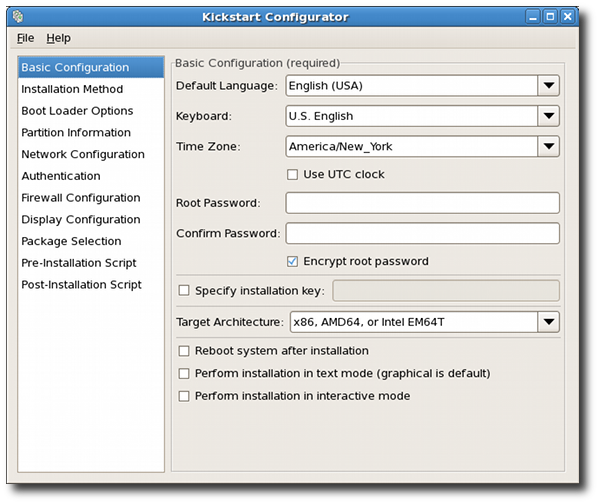
\includegraphics[scale=0.5]{./img/kickstart.png}\end{center}
.......................

\section{Rembo}
Rembo est le successeur de BPBatch. C’est un environnement commercial de création et de déploiement d’images sur PC. Le serveur Rembo peut s’exécuter sur Windows, Linux, ou encore FreeBSD et s’appuie sur un serveur DHCP. Les machines clientes doivent donc supporter PXE. Les clients du réseau sont répartis en plusieurs groupes, ce qui permet de définir des comportements par type de machine, par salle, ... 

\chapter{Sources}
http://fai-project.org/\\
http://www.markus-gattol.name/ws/fai.html\\
https://github.com/faiproject/fai\\
https://www.linux-magazine.com/w3/issue/100/066-071\_FAI.pdf\\
http://grml.org/\\


\end{document}
